\chapter{Quadratic Reciprocity}\label{chapter:quadratic-reciprocity}

\section{The Quadratic Character of 2}

In this section we consider the question for which odd primes $p$ we have that $2$ is a quadratic residue. By \zcref{exercise:uniform-legendre-exponent}, this is equivalent to the question for which primes $p$ we have
\begin{equation*}
  \frac{p-1}{\ord_p(2)}\equiv 0\pmod{2}.
\end{equation*}
In the following table we list the quantity $\frac{p-1}{\ord_p(2)}$ for the odd primes below $50$:
\begin{center}
  \begin{tabular}{c|ccccccccccccccc}
    $p$ & $3$ & $5$ & $7$ & $11$ & $13$ & $17$ & $19$ & $23$ & $29$ & $31$ & $37$ & $41$ & $43$ & $47$ \\ \midrule
    $\frac{p-1}{\ord_p(2)}$ & $1$ & $1$ & $2$ & $1$ & $1$ & $2$ & $1$ & $2$ & $1$ & $6$ & $1$ & $2$ & $3$ & $2$. \\
  \end{tabular}
\end{center}
This table shows that $2$ is a quadratic residue modulo $p$ for the primes
\begin{equation*}
  7,~17,~23,~31,~41,~47,~\ldots.
\end{equation*}
Unlike the case where we were seeking to characterize the primes for which $-1$ is a primitive root, these primes are not organized according to their residue class modulo $4$. The pattern is slightly more complicated. However, we may observe that the primes for which $2$ is a quadratic residue all happen to be close to a multiple of $8$, while the primes for which $2$ is a quadratic nonresidue are further from the multiples of $8$. This turns out to be the right idea: The number $2$ is a quadratic residue modulo $p$ if and only if $p$ is of the form $8k\pm 1$.

Note also that $2$ is a primitive root if and only if $\ord_p(2) = p-1$, so we see from the previous table that $2$ is a primitive root modulo $p$ for the primes
\begin{equation*}
  3,~5,~11,~13,~19,~29,~37,~\ldots.
\end{equation*}
However, it is not quite true that $2$ is a primitive root modulo $p$ whenever it is a quadratic nonresidue modulo $p$: The first prime for which $2$ is neither a quadratic residue nor a primitive root is $43$.

\begin{theorem}\label{theorem:second-supplement}
  The Legendre symbol of $2$ modulo $p$ satisfies the identity
  \begin{equation*}
    \legendre{2}{p}=(-1)^{\frac{p^2-1}{8}}.
  \end{equation*}
  In other words, $2$ is a quadratic residue if and only if $p\equiv \pm1\pmod{8}$, and it is a quadratic nonresidue if and only if $p\equiv \pm 3\pmod{8}$.
\end{theorem}

  Before we start the proof, recall that one of the proofs of \zcrefnamed{theorem:fermats-little-theorem} was obtained by multiplying all the numbers $1,\ldots,p-1$ with an integer $a$ to obtain the congruence
  \begin{equation*}
    a^{p-1}(p-1)!\equiv (p-1)!\pmod{p}.
  \end{equation*}
  Since $(p-1)!$ isn't divisible by $p$, it is invertible modulo $p$ and thus we found that $a^{p-1}\equiv 1\pmod{p}$.

\begin{proof}
  In this proof, we will write $P:=\frac{p-1}{2}$ so that $2P=p-1$. By \zcrefnamed{theorem:eulers-criterion} we have $\legendre{2}{p}\equiv 2^P\pmod{p}$, which gives us the congruences
  \begin{equation*}
    {\textstyle \legendre{2}{p}P!}\equiv 2^{P}P! \equiv 2\cdot 4 \cdot \cdots \cdot (2P) \pmod{p}
  \end{equation*}
  We proceed by carefully analyzing this product of all the even positive integers below $p$. If we define the numbers
  \begin{equation*}
    s:=\left\lfloor\frac{p-1}{4}\right\rfloor\qquad\text{and}\qquad t:=\left\lfloor\frac{p+1}{4}\right\rfloor,
  \end{equation*}
  so that $s+t=P$, then we can partition the set of all even positive integers below $p$ into two subsets
  \begin{equation*}
    S:=\{2k\mid 1\leq k \leq s\}\qquad\text{and}\qquad T:=\{2k\mid s+1\leq k\leq P\},
  \end{equation*}
  so that $S$ consists precisely of all the even positive integers up to and possibly including $P$, and $T$ consists of all the larger even integers up to and including $2P$. Note that the set $S$ has $s$ elements and the set $T$ has exactly $t$ elements.

  The key observation is that for every integer $y$ in $T$ there is a unique \emph{odd} integer $1\leq x\leq P$ so that $y=p-x$, which determines a bijection. Thus, taking the product modulo $p$ of all the even integers up to $p$ amounts to taking the product of all the integers $1\leq x\leq P$ with a sign change for every odd integer, of which there are $t$. In other words, we have the congruence
  \begin{equation*}
    {\textstyle \legendre{2}{p}P!}\equiv 2\cdot 4\cdot\cdots\cdot 2P\equiv (-1)^{t} P!\pmod{p}.
  \end{equation*}
  Since $P!$ is not divisible by $p$ we apply the cancellation law to obtain
  \begin{equation*}
    \legendre{2}{p}=(-1)^{t}.
  \end{equation*}
  We conclude the proof by observing that the parity of $t$ is determined according to the following cases:
  \begin{equation*}
    t\equiv
    \begin{cases}
      0\pmod{2} & \text{if }p\equiv \pm 1\pmod{8} \\
      1\pmod{2} & \text{if }p\equiv \pm 3\pmod{8}. \\
    \end{cases}
    \qedhere
  \end{equation*}
\end{proof}

The previous theorem is also known as the \emph{Second Supplement} of the law of Quadratic Reciprocity. An immediate corollary of the second supplement is that
\begin{equation*}
  \legendre{-2}{p}=\legendre{-1}{p}\legendre{2}{p}=
  \begin{cases}
    1 & \text{if }p\equiv 1\text{ or }3 \pmod{8} \\
    -1 & \text{if }p\equiv 5\text{ or }7\pmod{8}.
  \end{cases}
\end{equation*}

Since primitive roots are always quadratic nonresidues, we obtain the following corollary. Artin conjectured that there are infinitely many primes $p$ for which $2$ is a primitive root. More generally, he conjectured that for any integer $a$ that is neither $-1$ nor a perfect square, there are infinitely many primes for which $a$ is a primitive root.

\begin{corollary}
  If $2$ is a primitive root modulo $p$, then $p\equiv\pm 3\pmod{8}$.
\end{corollary}

\begin{table}[t]
  \centering
  \begin{tabular}{r|ccccccccccccccc}
          & 1\supst{}  & 2\supnd{}  & 3\suprd{}  & 4\supth{}  & 5\supth{}  & 6\supth{}   & 7\supth{}   & 8\supth{}   & 9\supth{}   & 10\supth{}  \\ \midrule
    $r=1$ & $17$ & $41$ & $73$ & $89$ & $97$ & $113$ & $137$ & $193$ & $233$ & $241$ \\
    $r=3$ & $3$  & $11$ & $19$ & $43$ & $59$ & $67$  & $83$  & $107$ & $131$ & $139$ \\
    $r=5$ & $5$  & $13$ & $29$ & $37$ & $53$ & $61$  & $101$ & $109$ & $149$ & $157$ \\
    $r=7$ & $7$  & $23$ & $31$ & $47$ & $71$ & $79$  & $103$ & $127$ & $151$ & $167$ \\
  \end{tabular}
  \caption[The first ten primes in each residue class modulo $8$]{\label{table:primes-congruent-to-r-mod-8}The first ten primes congruent to $r$ modulo $8$, for $r=1,3,5,7$.}
\end{table}

The second supplement can be used to show that there are infinitely many primes of the form $8k+r$ for any odd number $0<r<8$. We have already seen in \zcref{theorem:infinitude-of-primes-1-mod-power-of-2} that there are infinitely many primes congruent to $1$ modulo $2^n$. In particular, there are infinitely many primes of the form $8k+1$. It remains prove the analogous claims for the residue classes $3$, $5$, and $7$ modulo $8$. We will be following \Sierpinski{} \cite{sierpinski1988}. The first ten primes congruent to $r$ moduo $8$ for each odd residue class $r$ are given in \zcref{table:primes-congruent-to-r-mod-8}.

\begin{theorem}
  There are infinitely many primes congruent to $3$ modulo $8$.
\end{theorem}

\begin{proof}
  If $a$ is an odd integer, then $a^2\equiv 1\pmod{8}$ so that
  \begin{equation*}
    N_a := a^2+2
  \end{equation*}
  is congruent to $3$ modulo $8$. Not all prime divisors of $N_a$ can be congruent to $\pm 1$ modulo $8$, since if they were, then $N_a$ would likewise be congruent to $\pm 1$ modulo $8$. Therefore $N_a$ has a prime divisor $q$ so that
  \begin{equation*}
    q\equiv \pm{3}\pmod{8}.
  \end{equation*}
  Since $q\mid a^2+2$, it follows that $-2$ is a quadratic residue modulo $q$, so $q\nequiv-3\pmod{8}$. Thus it follows that $q\equiv 3\pmod{8}$.

  For a suitable choice of $a$, let $p_n$ be the $n$\supth{} prime number, so that $p_1=2$, $p_2=3$, $p_3=5$ and so forth. Then we define
  \begin{equation*}
    a=p_2p_3\cdots p_n,
  \end{equation*}
  so that any prime divisor of $N_a$ is larger than $p_n$. Since $N_a$ has a prime divisor congruent to $3$ modulo $8$, it follows that there are arbitrarily large such primes.
\end{proof}

\begin{theorem}
  There are infinitely many primes congruent to $5$ modulo $8$.
\end{theorem}

\begin{proof}
  If $a$ is an odd integer, then $a^2\equiv 1\pmod{8}$ so that
  \begin{equation*}
    N_a := a^2+4
  \end{equation*}
  is congruent to $5$ modulo $8$. As before, there must be a prime divisor $q$ of $N_a$ so that
  \begin{equation*}
    q\equiv \pm{3}\pmod{8}.
  \end{equation*}
  Since $q\mid a^2+4$, it follows that $-4$ is a quadratic residue modulo $q$. This implies that $-1$ is a quadratic residue modulo $q$, so that $q\equiv 1\pmod{4}$. Since we assumed that $q\nequiv 1\pmod{8}$, it follows that $q\equiv -3\pmod{8}$.

  For a suitable choice of $a$, define
  \begin{equation*}
    a=p_2p_3\cdots p_n
  \end{equation*}
  so that any prime divisor of $N_a$ is larger than $p_n$. Since $N_a$ has a prime divisor congruent to $5$ modulo $8$, it follows that there are arbitrarily large such primes.
\end{proof}

\begin{theorem}
  There are infinitely many primes congruent to $7$ modulo $8$.
\end{theorem}

\begin{proof}
  The idea of the proof is to find a natural number $N$ of the form
  \begin{equation*}
    N=2a^2-b^2,
  \end{equation*}
  so that $N\equiv -1\pmod{8}$ and $N$ is relatively prime to any $m \leq n$. Assuming that $n>1$, a suitable choice of $a$ and $b$ is $a:=n!$ and $b:=1$. Indeed, in this case $a$ is even, so that $2a^2-1\equiv -1\pmod{8}$.

  Under these assumptions, $N$ will have a prime factor $q\nequiv 1\pmod{8}$, and furthermore we will have
  \begin{equation*}
    2a^2 \equiv b^2\pmod{q}.
  \end{equation*}
  Since $a^2$ and $b^2$ are clearly quadratic residues modulo $q$, it follows that $2$ is a quadratic residue, implying that $q\equiv\pm 1\pmod{8}$. However, since we have chosen $q$ so that $q\nequiv 1\pmod{8}$, it follows that $q\equiv -1\pmod{8}$. Furthermore, since $q$ is relatively prime to any $m \leq n$, it follows that $n<q$, which shows that there are arbitrarily large primes $q\equiv -1\pmod{8}$.
\end{proof}

\section{The Statement of Quadratic Reciprocity}

We have already established several facts about Legendre symbols. The Legendre symbol is multiplicative, meaning that
\begin{equation*}
  \legendre{ab}{p}=\legendre{a}{p}\legendre{b}{p}.
\end{equation*}
The Legendre symbol $\legendre{-1}{p}$ can be computed according to whether $p$ is congruent to $1$ or $3$ modulo $4$:
\begin{equation*}
  \legendre{-1}{p}=
  \begin{cases}
    1 & \text{if }p\equiv 1\pmod{4}\\
    -1 & \text{if }p\equiv 3\pmod{4}.
  \end{cases}
\end{equation*}
The Legendre symbol $\legendre{2}{p}$ can likewise be computed according to whether $p$ is congruent to $\pm 1$ or $\pm 3$ modulo $8$:
\begin{equation*}
  \legendre{2}{p}=
  \begin{cases}
    1 & \text{if }p\equiv \pm1\pmod{8}\\
    -1 & \text{if }p\equiv \pm3\pmod{8}.
  \end{cases}
\end{equation*}
We need one final piece to effectively compute Legendre symbols: a way to determine the Legendre symbol $\legendre{q}{p}$ when $q$ is an odd prime. The recipe for determining $\legendre{q}{p}$ is given by the law of quadratic reciprocity.

To build some intuition for what the law of quadratic reciprocity should assert, we recall from \zcref{exercise:uniform-legendre-exponent} that the Legendre symbol of $a$ modulo $p$ can be computed by
\begin{equation*}
  \legendre{a}{p}=(-1)^{\frac{p-1}{\ord_p(a)}}.
\end{equation*}
Thus, the Legendre symbol of $a$ modulo $p$ depends only of the parity of the quantity
\begin{equation*}
  \frac{p-1}{\ord_p(a)},
\end{equation*}
which gives us a fairly quick way of determining the Legendre symbol $\legendre{q}{p}$ for small odd primes $p$ and $q$. We listed signs of the Legendre symbols of $q$ modulo $p$ in \zcref{table:legendre-symbols-distinct-odd-primes}.

\begin{table}[t]
  \begin{center}
    \begin{tabular}{c|cccccccccc}
      \toprule
      $p \backslash q$ & $3$ & $5$ & $7$ & $11$ & $13$ & $17$ & $19$ & $23$ & $29$ & $31$ \\
      \midrule
      $3$  &  & $-$ & $+$ & $-$ & $+$ & $-$ & $+$ & $-$ & $-$ & $+$ \\
      $5$  & $-$ &  & $-$ & $+$ & $-$ & $-$ & $+$ & $-$ & $+$ & $+$ \\
      $7$  & $-$ & $-$ &  & $+$ & $-$ & $-$ & $-$ & $+$ & $+$ & $-$ \\
      $11$ & $+$ & $+$ & $-$ &  & $-$ & $-$ & $-$ & $+$ & $-$ & $+$ \\
      $13$ & $+$ & $-$ & $-$ & $-$ &  & $+$ & $-$ & $+$ & $+$ & $-$ \\
      $17$ & $-$ & $-$ & $-$ & $-$ & $+$ &  & $+$ & $-$ & $-$ & $-$ \\
      $19$ & $-$ & $+$ & $+$ & $+$ & $-$ & $+$ &  & $+$ & $-$ & $-$ \\
      $23$ & $+$ & $-$ & $-$ & $-$ & $+$ & $-$ & $-$ &  & $+$ & $+$ \\
      $29$ & $-$ & $+$ & $+$ & $-$ & $+$ & $-$ & $-$ & $+$ &  & $-$ \\
      $31$ & $-$ & $+$ & $+$ & $-$ & $-$ & $-$ & $+$ & $-$ & $-$ &  \\
      \bottomrule
    \end{tabular}
    \caption[The sign of the Legendre symbol]{\label{table:legendre-symbols-distinct-odd-primes}The sign of the Legendre symbol $\legendre{q}{p}$, ranging over pairs of distinct odd primes $p$ and $q$.}
  \end{center}
\end{table}

The patterns in this table might not be immediately apparent. However, those who did \zcref{exercise:legendre-5} might spot that column $5$ is identical to row $5$. Looking for more identical columns and rows, we create a new table by comparing the entry in row $i$ and column $j$ in \zcref{table:legendre-symbols-distinct-odd-primes} with the entry in row $j$ and column $i$. When these two entries are equal, we mark it with a solid black circle (\tikz[baseline=-.58ex] \fill (0,0) circle (0.9ex);), and if they are different we mark it with an open circle (\tikz[baseline=-.58ex] \draw (0,0) circle (0.9ex);). This results in the following table:

\begingroup
\newcommand{\yes}{\tikz[baseline=-.58ex] \fill (0,0) circle (0.9ex);}
\newcommand{\no}{\tikz[baseline=-.58ex] \draw (0,0) circle (0.9ex);}

\begin{table}[h]
  \begin{center}
    \begin{tabular}{c|cccccccccc}
      \toprule
      $p \backslash q$ & $3$ & $5$ & $7$ & $11$ & $13$ & $17$ & $19$ & $23$ & $29$ & $31$ \\
      \midrule
      $3$  &  & $\yes$ & $\no$ & $\no$ & $\yes$ & $\yes$ & $\no$ & $\no$ & $\yes$ & $\no$ \\
      $5$  & $\yes$ &  & $\yes$ & $\yes$ & $\yes$ & $\yes$ & $\yes$ & $\yes$ & $\yes$ & $\yes$ \\
      $7$  & $\no$ & $\yes$ &  & $\no$ & $\yes$ & $\yes$ & $\no$ & $\no$ & $\yes$ & $\no$ \\
      $11$ & $\no$ & $\yes$ & $\no$ &  & $\yes$ & $\yes$ & $\no$ & $\no$ & $\yes$ & $\no$ \\
      $13$ & $\yes$ & $\yes$ & $\yes$ & $\yes$ &  & $\yes$ & $\yes$ & $\yes$ & $\yes$ & $\yes$ \\
      $17$ & $\yes$ & $\yes$ & $\yes$ & $\yes$ & $\yes$ &  & $\yes$ & $\yes$ & $\yes$ & $\yes$ \\
      $19$ & $\no$ & $\yes$ & $\no$ & $\no$ & $\yes$ & $\yes$ &  & $\no$ & $\yes$ & $\no$ \\
      $23$ & $\no$ & $\yes$ & $\no$ & $\no$ & $\yes$ & $\yes$ & $\no$ &  & $\yes$ & $\no$ \\
      $29$ & $\yes$ & $\yes$ & $\yes$ & $\yes$ & $\yes$ & $\yes$ & $\yes$ & $\yes$ &  & $\yes$ \\
      $31$ & $\no$ & $\yes$ & $\no$ & $\no$ & $\yes$ & $\yes$ & $\no$ & $\no$ & $\yes$ &  \\
      \bottomrule
    \end{tabular}
  \end{center}
\end{table}
\endgroup

Using this table, we quickly spot that columns $5$, $13$, $17$, and $29$ are identical to rows $5$, $13$, $17$, and $29$, respectively, which means that these columns were also identical to their respective rows in \zcref{table:legendre-symbols-distinct-odd-primes}. Something special is going on with the primes
\begin{equation*}
  5,~13,~17,~29,
\end{equation*}
and something seems to be off about the primes
\begin{equation*}
  3,~7,~11,~19,~23,~31.
\end{equation*}
We are very familiar with this grouping of the primes by now: The first set of primes are all congruent to $1$ modulo $4$, while the second set of primes are all congruent to $3$ modulo $4$. These observations suggest the following:
\begin{enumerate}
\item If at least one of $p$ and $q$ is congruent to $1$ modulo $4$, then we have
  \begin{equation*}
    \legendre{q}{p}=\legendre{p}{q}.
  \end{equation*}
\item If both $p$ and $q$ are congruent to $3$ modulo $4$, then we have
  \begin{equation*}
    \legendre{q}{p}=-\legendre{p}{q}.
  \end{equation*}
\end{enumerate}
Legendre and Gauss spotted these patterns towards the end of the 18th century. They formulated it succinctly as follows:

\begin{theorem}[The Law of Quadratic Reciprocity]\label{theorem:quadratic-reciprocity}
  For any two distinct odd primes $p$ and $q$ we have
  \begin{equation*}
    \legendre{q}{p}\legendre{p}{q}=(-1)^{\frac{p-1}{2}\frac{q-1}{2}}.
  \end{equation*}
\end{theorem}

\begin{example}
  The law of quadratic reciprocity is incredibly effective in computations of Legendre symbols. For example, since $17$ and $101$ are congruent to $1$ modulo $4$, we have
  \begin{equation*}
    \legendre{17}{101}=\legendre{101}{17}=\legendre{16}{17}=\legendre{4}{17}\legendre{4}{17}=1.
  \end{equation*}
  Indeed, it turns out that $44^2\equiv 17$ and $57^2\equiv17$ modulo $101$.

  On the other hand, both $23$ and $43$ are congruent to $3$ modulo $4$, so the law of quadratic reciprocity tells us that
  \begin{equation*}
    \legendre{23}{43}=-\legendre{43}{23}=-\legendre{20}{23}=-\legendre{4}{23}\legendre{5}{23}=-\legendre{5}{23}=-\legendre{23}{5}=-\legendre{3}{5}=1.
  \end{equation*}
  In this case, it turns out that $18^2\equiv 23$ and $25^2\equiv 23$ modulo $43$.
  
  As a final example, for good measure, note that $31$ and $83$ are both congruent to $3$ modulo $4$. Using the law of quadratic reciprocity we obtain that
  \begin{equation*}
    \legendre{31}{83}=-\legendre{83}{31}=-\legendre{21}{31}=-\legendre{3}{31}\legendre{7}{31}=-\legendre{31}{3}\legendre{31}{7}=-\legendre{1}{3}\legendre{3}{7}=\legendre{7}{3}=1.
  \end{equation*}
\end{example}

The quadratic residuosity of an odd prime $q$ modulo a distinct odd prime $p$ determines some important restrictions on the form of the prime $p$. We spell these out in the following theorem, which is essentially a reformulation of the law of quadratic reciprocity.
  
\begin{theorem}
  Consider two distinct odd primes $p$ and $q$. The following two statements hold:
  \begin{enumerate}
  \item \label{itemi:explicit-reciprocity}If $p\equiv 1\pmod{4}$, then $q$ is a quadratic residue modulo $p$ if and only if there exists an odd integer $0<a<q$ such that
    \begin{equation*}
      p\equiv a^2\pmod{4q}.
    \end{equation*}
  \item \label{itemii:explicit-reciprocity}If $p\equiv 3\pmod{4}$, then $q$ is a quadratic residue modulo $p$ if and only if there exists an odd integer $0<a<q$ such that
    \begin{equation*}
      p\equiv -a^2\pmod{4q}.
    \end{equation*}
  \end{enumerate}
\end{theorem}

\begin{proof}
  Before proving each statement, we note that for any $u\nequiv 0\pmod{q}$, if the quadratic congruence
  \begin{equation*}
    x^2\equiv u\pmod{q}
  \end{equation*}
  is solvable, then it has two solutions. Of these two solutions, one is even and the other is odd. Thus, if it is solvable, we can always pick an odd solution.
  
  For the first claim of the theorem, assume that $p\equiv 1\pmod{4}$. By the law of quadratic reciprocity, it follows that
  \begin{equation*}
    \legendre{q}{p}=\legendre{p}{q}. 
  \end{equation*}
  Furthermore, $\legendre{p}{q}=1$ if and only if there exists an odd integer $0<a<q$ such that $p\equiv a^2\pmod{q}$. Furthermore, since $a$ is odd and $p\equiv 1\pmod{4}$, it also follows that $p\equiv a^2\pmod{4}$. Thus we see that $\legendre{q}{p}=1$ if and only if there exists an odd integer $0<a<q$ such that
  \begin{equation*}
    p\equiv a^2\pmod{4q}.
  \end{equation*}
  
  For the second claim, assume that $p\equiv 3\pmod{4}$. By the law of quadratic reciprocity, it follows that
  \begin{equation*}
    \legendre{q}{p}\legendre{p}{q}=(-1)^{\frac{p-1}{2}\frac{q-1}{2}}=(-1)^{\frac{q-1}{2}}=\legendre{-1}{q}.
  \end{equation*}
  By rearranging the terms, we find that $\legendre{q}{p}=\legendre{-p}{q}$, and thus there is an odd integer $a$ such that
  \begin{equation*}
    p\equiv -a^2\pmod{q}.
  \end{equation*}
  Since $a$ is assumed to be odd and $p\equiv 3\pmod{4}$, we find furthermore that $-a^2\equiv p\pmod{4}$. We conclude that $\legendre{q}{p}=1$ if and only if there is an odd integer $0<a<q$ such that
  \begin{equation*}
    p\equiv -a^2\pmod{4q}.\qedhere
  \end{equation*}
\end{proof}

The previous theorem can be used at once to characterize the primes $p$ for which $3$ is a quadratic residue modulo $p$. Taking $q=3$ in the previous theorem, we find that $3$ is a quadratic residue modulo $p$ if and only if $p$ is of the form $12k\pm 1$, since the only odd quadratic residue modulo $3$ is $1$. For any odd prime $p\neq 3$, we have thus shown that
\begin{equation*}
  \legendre{3}{p}=
  \begin{cases}
    1 & \text{if }p\equiv \pm 1\pmod{12}, \\
    -1 & \text{if }p\equiv \pm 5\pmod{12}.
  \end{cases}
\end{equation*}
Likewise, we can characterize the primes $p$ for which $5$ is a quadratic residue modulo $p$. Taking $q=5$ in the previous theorem, we find that $5$ is a quadratic residue modulo $p$ if and only if $p$ is of the form $20k\pm 1$ or $20k\pm 9$, since the two odd squares modulo $5$ are $1^2$ and $3^2$. For any odd prime $p\neq 5$, we have thus shown that
\begin{equation*}
  \legendre{5}{p}=
  \begin{cases}
    1 & \text{if }p\equiv \pm 1\pmod{10}, \\
    -1 & \text{if }p\equiv \pm 3\pmod{10}.
  \end{cases}
\end{equation*}

\section{Gauss's Lemma}

While it is customary to consider the standard residue classes modulo an odd prime $p$ to be the integers $0\leq r<p$, we have now the occasion to consider the complete residue system of integers between $-\frac{p-1}{2}$ and $\frac{p-1}{2}$.

\begin{definition}
  The \emph{least absolute residue} of an integer $a$ modulo a natural number $n$ is the unique integer
  \begin{equation*}
    -\frac{n}{2} < x \leq \frac{n}{2}
  \end{equation*}
  such that $x\equiv a\pmod{n}$. We will write $\lres{a}{n}$ for the least absolute residue of $a$ modulo $n$, and we will write $\abslres{a}{n}$ for its absolute value.
\end{definition}

Thus, the least absolute residue of an integer $a$ modulo an odd prime $p$, which is what we will be using this concept for, is the unique integer
\begin{equation*}
  -\frac{p-1}{2}\leq x\leq \frac{p-1}{2}
\end{equation*}
such that $x\equiv a\pmod{p}$. For example, the least absolute residue of $4$ modulo $7$ is $-3$, the least absolute residue of $6$ modulo $13$ is $6$, and the least absolute residue of $12$ modulo $13$ is $-1$. In the following table, we list the least absolute residues modulo $11$:
\begin{center}
  \begin{tabular}{c|ccccccccccc}
    $a$ & $0$ & $1$ & $2$ & $3$ &  $4$ & $5$ & $6$ & $7$ & $8$ & $9$ & $10$ \\ \midrule
    $\lres{a}{11}$ & $0$ & $1$ & $2$ & $3$ &  $4$ & $5$ & $-5$ & $-4$ & $-3$ & $-2$ & $-1$.
  \end{tabular}
\end{center}

If we consider an integer $a$ relatively prime to an odd prime $p$, then multiplication by $a$ defines a bijection on $\mathbb{Z}/p\mathbb{Z}$. It follows that the function
\begin{equation*}
  x\mapsto \lres{ax}{p} : \bigl\{0,\ldots,p-1\bigr\}\to\bigl\{-\tfrac{p-1}{2},\ldots,\tfrac{p-1}{2}\bigr\}
\end{equation*}
is also a bijection. Restricting this bijection to the set $\{1,\ldots,\frac{p-1}{2}\}$, we obtain an injective function
\begin{equation*}
  x\mapsto \lres{ax}{p} :\bigl\{1,\ldots,\tfrac{p-1}{2}\bigr\}\to\bigl\{-\tfrac{p-1}{2},\ldots,\tfrac{p-1}{2}\bigr\}.
\end{equation*}
The following lemma shows that every $1\leq x\leq\frac{p-1}{2}$ occurs exactly once as the absolute value of any number of the form $\lres{ax}{p}$.

\begin{lemma}\label{lemma:bijection-gausss-lemma}
  The function
  \begin{equation*}
    r_a:\bigl\{1,\ldots,\tfrac{p-1}{2}\bigr\}\to\bigl\{1,\ldots,\tfrac{p-1}{2}\bigr\}
  \end{equation*}
  given by $r_a(x):=\abslres{ax}{p}$ is a bijection.
\end{lemma}

\begin{proof}
  Since $r_a$ is a function between two sets of finite size $\frac{p-1}{2}$, it suffices to show that $r_a$ is injective. To this end, consider $x$ and $y$ such that $r_a(x)=r_a(y)$. Since the function $x\mapsto \lres{ax}{p}$ is injective, this implies that
  \begin{equation*}
    \lres{ax}{p}=-\lres{ay}{p}
  \end{equation*}
  or, equivalently, that $ax-ay$ is divisible by $p$. Since $a$ is relatively prime to $p$, this implies that $x-y$ is divisible by $p$, i.e., that $x=y$.
\end{proof}

\begin{lemma}[Gauss's Lemma]\label{lemma:gausss-lemma}
  Consider an odd prime $p$ and an integer such that $p\nmid a$. Define $\mu$ to be the number of elements $x$ among the residue classes
  \begin{equation*}
    a,~2a,~3a,~\ldots,~\tfrac{p-1}{2}a\pmod{p},
  \end{equation*}
  such that $\lres{ax}{p}$ is negative. Then we have
  \begin{equation*}
    \legendre{a}{p}=(-1)^\mu.
  \end{equation*}
\end{lemma}

\begin{proof}
  Write $P:=(p-1)/2$. Then we have that $p\nmid P!$, so suffices to show that
  \begin{equation*}
    \legendre{a}{p}P!\equiv (-1)^\mu P!\pmod{p}.
  \end{equation*}
  By \zcrefnamed{theorem:eulers-criterion} we have $\legendre{a}{p}\equiv a^{P}\pmod{p}$, so we obtain that
  \begin{equation*}
    \legendre{a}{p}P!\equiv a^P P! \pmod{p}.
  \end{equation*}
  Redistributing the $P$ factors of $a$ of the exponent $a^P$ over $P!$, and using \zcref{lemma:gausss-lemma}, we obtain:
  \begin{equation*}
    a^P P! = (1a)(2a)\cdots(Pa) \equiv (-1)^\mu P! \pmod{p}.\qedhere
  \end{equation*}
\end{proof}

\section[Eisenstein's Proof]{Eisenstein's Proof of the Law of Quadratic Reciprocity}

Gauss was the first to prove the law of quadratic reciprocity in 1796, when he was only 19 years old. This proof was included in his seminal work, \emph{Disquisitiones Arithmeticae}, published in 1801. Gauss was very fond of this result, and throughout his life-time he would publish seven different proofs.

The proof we will present here is due to Gotthold Eisenstein, which he published in 1844. It is celebrated for its simplicity and for the insightful perspective it provides on geometric aspects of the quadratic reciprocity law.

In Eisenstein's proof of the law of quadratic reciprocity, we will make use of the \emph{floor function} $x\mapsto \lfloor x\rfloor$, which is a function from the rational numbers or the real numbers, to the integers. The integer
\begin{equation*}
  \lfloor x\rfloor
\end{equation*}
is the largest integer below $x$. In other words, its defining property is that the floor function satisfies the logical equivalence
\begin{equation*}
  k\leq \lfloor x\rfloor\qquad\Leftrightarrow \qquad k\leq x
\end{equation*}
for every integer $k$ and every rational or real number $x$. Concretely, we have the following examples:
\begin{equation*}
  \left\lfloor\frac{3}{2}\right\rfloor=1,\qquad \left\lfloor\frac{29}{31}\right\rfloor=0,\qquad\text{and}\qquad\left\lfloor-\frac{1}{4}\right\rfloor=-1.
\end{equation*}

\begin{proof}[Eisenstein's Proof of \zcrefnamed{theorem:quadratic-reciprocity}]
  By \zcrefnamed{lemma:gausss-lemma} it suffices to show that
  \begin{equation*}
    (-1)^{\mu(q,p)}(-1)^{\mu(p,q)}=(-1)^{\frac{p-1}{2}\frac{q-1}{2}}.
  \end{equation*}
  In other words, we have to show that
  \begin{equation*}
    \mu(q,p)+\mu(p,q)\equiv \frac{p-1}{2}\frac{q-1}{2}\pmod{2}.
  \end{equation*}
  This suggests that there should be a way of splitting a set of $\frac{p-1}{2}\frac{q-1}{2}$ points into two subsets $S$ and $T$, so that their respective number of elements have the same parities as the quantities $\mu(q,p)$ and $\mu(p,q)$. There is indeed such a way. \zcref{figure:eisenstein-quadratic-reciprocity} shows Eisenstein's setup in case of the primes $p=17$ and $q=13$. 
  
  \begin{figure}[t]
    \centering
    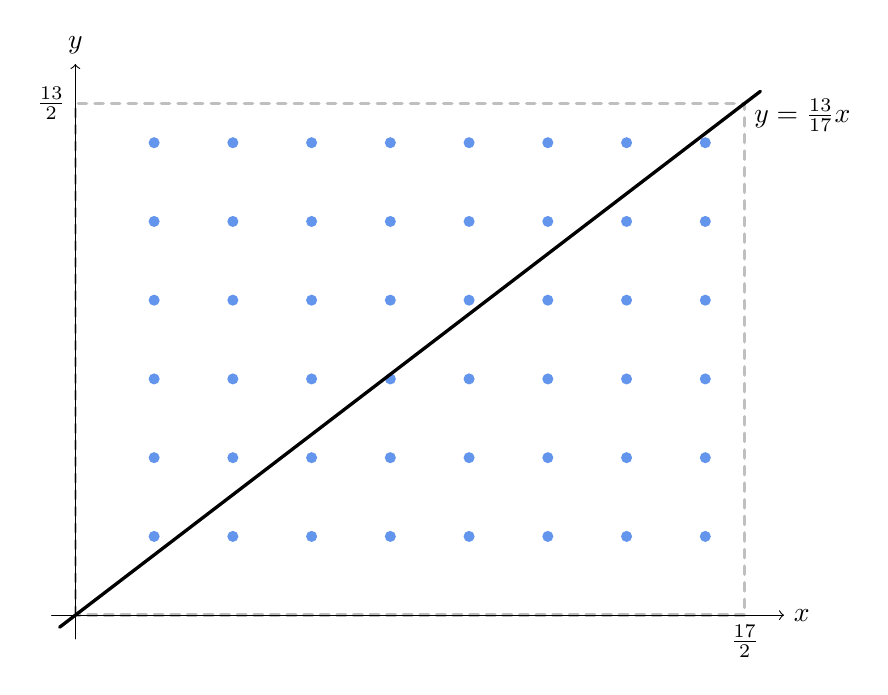
\begin{tikzpicture}[scale=1,line join=round,line cap=round]
      
      % Define primes and half-values
      \def\p{17}
      \def\q{13}
      \def\xmax{8.5} % q/2
      \def\ymax{6.5} % p/2
      
      % Draw the rectangle boundaries (0,0) to (q/2, p/2)
      \draw[very thick,lightgray,dashed] (0,0) rectangle (\xmax,\ymax);

            % Draw coordinate axes
      \draw[->] (-0.3,0) -- (\xmax+0.5,0) node[right] {$x$};
      \draw[->] (0,-0.3) -- (0,\ymax+0.5) node[above] {$y$};
      
      \node[below] at (\xmax,0) {$\frac{17}{2}$};
      \node[left] at (0,\ymax) {$\frac{13}{2}$};
      
      % Draw the lattice points (integer coordinates inside the rectangle)
      \foreach \x in {1,2,3,4,5,6,7,8} {
        \foreach \y in {1,2,...,6} {
          \fill[CornflowerBlue] (\x,\y) circle (2pt);
        }
      }
      
      \draw[very thick, domain=-0.2:\xmax+0.2] plot (\x, {(\q/\p)*\x});
      
      \node[right,yshift=-1ex] at (\xmax,\ymax) {$y=\frac{13}{17}x$};    
    \end{tikzpicture}
    \caption[Eisenstein's proof of quadratic reciprocity]{\label{figure:eisenstein-quadratic-reciprocity}In Eisenstein's proof of quadratic reciprocity, we count the $\frac{p-1}{2}$ by $\frac{q-1}{2}$ lattice points in the marked rectangle as the sum of the number lattice points below the diagonal and the number of lattice points above the diagonal.}
  \end{figure}  
  
  Consider the set of $\frac{p-1}{2}$ by $\frac{q-1}{2}$ lattice points in the positive quadrant of the plane; that is, the points with positive integer coordinates within the rectangle spanned by the four points
  \begin{equation*}
    {\textstyle \bigl(0,0\bigr),~\bigl(\frac{p}{2},0\bigr),~\bigl(\frac{p}{2},\frac{q}{2}\bigr),~\text{and}~\bigl(0,\frac{q}{2}\bigr)}.
  \end{equation*}
  We partition these lattice points by the diagonal of the rectangle: The set of lattice points below the diagonal is $S$, and the set of lattice points above the diagonal is $T$. Since the diagonal of this rectangle is given by the line $y=\frac{q}{p}x$, there is no point with positive integer coordinates on the diagonal, so there is no ambiguity as to which part a lattice point belongs to.

  Now observe that the number $|S|$ of lattice points in the set $S$ is given by
  \begin{equation*}
    |S|= \sum_{k=1}^{\frac{p-1}{2}}\left\lfloor\frac{kq}{p}\right\rfloor.
  \end{equation*}
  This formula is obtained by first recognizing that for each $1\leq k\leq\frac{p-1}{2}$, a lattice point of the form $(k,i)$ is in the set $S$ if and only if
  \begin{equation*}
    1\leq i \leq \frac{q}{p}k.
  \end{equation*}
  The number of such lattice points is $\bigl\lfloor\frac{kq}{p}\bigr\rfloor$, so the total number of elements in $S$ is obtained by summing up all of these totals. Similarly, the number $|T|$ of lattice points in the set $T$ is given by
  \begin{equation*}
    |T|= \sum_{k=1}^{\frac{q-1}{2}}\left\lfloor\frac{kp}{q}\right\rfloor.
  \end{equation*}
  Thus, it remains to prove that
  \begin{equation*}
    \sum_{k=1}^{\frac{p-1}{2}}\left\lfloor\frac{kq}{p}\right\rfloor\equiv \mu(q,p)\pmod{2}\quad\text{and}\quad \sum_{k=1}^{\frac{q-1}{2}}\left\lfloor\frac{kp}{q}\right\rfloor\equiv\mu(p,q)\pmod{2}.
  \end{equation*}
  We will verify these congruences separately in the following lemma.
\end{proof}

\begin{lemma}
  Consider an odd prime $p$ and an odd integer $a$ not divisible by $p$, and let $\mu(a,p)$ be the quantity defined in \zcrefnamed{lemma:gausss-lemma}. Then
  \begin{equation*}
    \sum_{k=1}^{\frac{p-1}{2}}\left\lfloor\frac{ka}{p}\right\rfloor \equiv \mu(a,p)\pmod{2}.
  \end{equation*}
\end{lemma}

\begin{proof}
  For each $k$ there are unique integers $q_k$ and $r_k$ such that $ka=q_kp+r_k$, where
  \begin{equation*}
    -\frac{p-1}{2}\leq r_k\leq \frac{p-1}{2}.
  \end{equation*}
  It follows that
  \begin{equation*}
    \left\lfloor\frac{ka}{p}\right\rfloor=
    \begin{cases}
      q_k & \text{if }r_k>0\\
      q_{k}-1 & \text{if }r_k<0.
    \end{cases}
  \end{equation*}
  Adding up the integers $\lfloor\frac{ka}{p}\rfloor$ therefore amounts to adding up the integers $q_k$ and subtracting the number of integers $k$ such that $r_k$ is negative:
  \begin{equation*}
    \sum_{k=1}^{\frac{p-1}{2}}\left\lfloor\frac{ka}{p}\right\rfloor = \sum_{k=1}^{\frac{p-1}{2}}q_k-\mu(a,p).
  \end{equation*}
  To complete the proof, it therefore suffices to show that
  \begin{equation*}
    \sum_{k=1}^{\frac{p-1}{2}}q_k \equiv 0\pmod{2}.
  \end{equation*}

  To prove this, recall from \zcref{lemma:bijection-gausss-lemma} that the map $k\mapsto |r_k|$ is a permutation of the set $\{1,\ldots,\frac{p-1}{2}\}$. In other words, every integer from $1$ to $\frac{p-1}{2}$ occurs exactly once as an integer of the form $|r_k|$. Since the parity of an integer is unchanged by taking its absolute value, we have
  \begin{equation*}
    \sum_{k=1}^{\frac{p-1}{2}}r_k \equiv \sum_{k=1}^{\frac{p-1}{2}}|r_k| \equiv \sum_{k=1}^{\frac{p-1}{2}}k \pmod{2}.
  \end{equation*}
  On the other hand, observe that since $a$ and $p$ are assumed to be odd, we have the congruences
  \begin{equation*}
    k\equiv ka = q_kp + r_k \equiv q_k+r_k\pmod{2}.
  \end{equation*}
  Thus we obtain the congruences
  \begin{equation*}
    \sum_{k=1}^{\frac{p-1}{2}}k\equiv\sum_{k=1}^{\frac{p-1}{2}}q_k + \sum_{k=1}^{\frac{p-1}{2}}r_k \equiv\sum_{k=1}^{\frac{p-1}{2}}q_k + \sum_{k=1}^{\frac{p-1}{2}}k \pmod{2}.
  \end{equation*}
  Subtracting $\sum_k k$ from both sides, we find that $\sum_k q_k\equiv 0\pmod{2}$.
\end{proof}

\exercises

\begin{starter}
  \exercise Compute the values of the following Legendre symbols:
  \begin{equation*}
    \legendre{101}{163}, \quad \legendre{137}{359}, \quad \legendre{113}{479}, \quad\text{and}\quad \legendre{139}{953}.
  \end{equation*}
  \exercise Compute the values of the following Legendre symbols:
  \begin{equation*}
    \legendre{113}{131}, \quad \legendre{131}{311}, \quad\text{and}\quad \legendre{311}{113}.
  \end{equation*}
  \exercise Compute the values of the following Legendre symbols:
  \begin{equation*}
    \legendre{199}{919}, \quad \legendre{919}{991}, \quad\text{and}\quad \legendre{991}{199}.
  \end{equation*}
  \exercise Compute the values of the following Legendre symbols:
  \begin{equation*}
    \legendre{337}{373}, \quad \legendre{373}{733}, \quad\text{and}\quad \legendre{733}{337}.
  \end{equation*}
  \exercise Show that the system of congruences
  \begin{align*}
    x-y\equiv 1\pmod{p},\\
    xy\equiv 1\pmod{p}
  \end{align*}
  has a solution if and only if $p\equiv \pm 1\pmod{10}$.
  % \exercise Determine whether the following quadratic congruences have solutions:
  % \begin{subexenum}
  % \item $x^2+x+1\equiv 0\pmod{15}$.
  % \item $x^2 + x +4\equiv 0\pmod{15}$.
  % \item $3x^2+2x+5\equiv 0\pmod{24}$.
  % \item $3x^2 + 7x + 2\equiv 0\pmod{24}$.
  % \item $x^2 - 2x -8 \equiv 0 \pmod{35}$.
  % \item $x^2 + x -6\equiv 0\pmod{77}$.
  % \end{subexenum}
\end{starter}

\begin{routine}
  \exercise Consider a prime $p>3$. Show that
  \begin{equation*}
    \legendre{6}{p}=
    \begin{cases}
      1 & \text{if }p\equiv \pm 1,\pm 5\pmod{24}, \\
      -1 & \text{if }p\equiv \pm 7,\pm 11\pmod{24}.
    \end{cases}
  \end{equation*}
  \exercise Consider an odd prime $p\neq 5$. Show that
  \begin{equation*}
    \legendre{10}{p}=
    \begin{cases}
      1 & \text{if }p\equiv \pm 1,\pm3, \pm 9,\pm 13 \pmod{40}, \\
      -1 & \text{if }p\equiv \pm 7, \pm 11, \pm 17, \pm 19 \pmod{40}.
    \end{cases}
  \end{equation*}
  \exercise Determine whether the following quadratic congruences have solutions:
  \begin{subexenum}
  \item $x^2+x+1\equiv 0\pmod{13}$.
  \item $x^2+x+3\equiv 0\pmod{7}$.
  \item $2x^2+3x+5\equiv 0\pmod{17}$.
  \item $x^2+4x+8\equiv 0\pmod{23}$.
  \item $2x^2+3x+4\equiv 0\pmod{11}$.
  \item $4x^2 + 7x+14 \equiv 0\pmod{31}$.
  \end{subexenum}  
  \exercise Show that $2$ is a quadratic residue modulo any prime divisor of the $n$\supth{} Fermat number $F_n=2^{2^n}+1$, for $n\geq 2$.
  \exercise Consider a prime $p$ such that $q:=2p+1$ and $r:=2(2p+1)+1=4p+3$ are both prime. Prove that
  \begin{equation*}
    \ord_r(2)=q.
  \end{equation*}
\end{routine}

\begin{challenge}
  \exercise Show that if the $n$\supth{} Fermat number $F_n=2^{2^n}+1$ is prime, then $3$ is a primitive root modulo $F_n$.
  \exercise Consider an odd prime $p$. Show that the following are equivalent:
  \begin{enumerate}
  \item The Mersenne number $M_p=2^p-1$ has a common prime divisor with $2p+1$.
  \item The prime $p$ is a \emph{Sophie Germain prime}, meaning that the number $2p+1$ is prime, and furthermore $p\equiv 3\pmod{4}$.
  \end{enumerate}
  Conclude that
  \begin{equation*}
    M_{11},M_{23},M_{83},M_{131},M_{179},~\text{and}~M_{191}
  \end{equation*}
  are all composite.
  \exercise
  \begin{subexenum}
  \item Show that for any prime $p\equiv 3\pmod{4}$ greater than $3$, there exists a prime $q<p$ such that $p$ is a quadratic nonresidue modulo $q$.
  \item Show that for any prime $p\equiv 1\pmod{4}$, there exists a prime $q<p$ such that $p$ is a quadratic nonresidue modulo $q$. Hint: First show that there exists a quadratic nonresidue $0<a<p$ such that $a\equiv 1\pmod{4}$.
  \end{subexenum}
  \exercise
  \begin{subexenum}
  \item For any integer $a>2$, let $p$ be a prime factor of $a^4-a^2+1$. Show that
    \begin{equation*}
      \ord_p(a)=12.
    \end{equation*}
  \item Use a suitable choice of $a$ in
    \begin{equation*}
      N_a:=a^6+1
    \end{equation*}
    to show that there are infinitely many primes congruent to $1$ modulo $12$.
  \item For each $r$ in the set $\{5,7,11\}$, show that there are infinitely many primes congruent to $r$ modulo $12$.    
  \end{subexenum}
\end{challenge}


%%% Local Variables:
%%% mode: latex
%%% TeX-master: "number-theory"
%%% TeX-engine: luatex
%%% End:
